\documentclass[twocolumn,10pt]{article}

\usepackage[T1]{fontenc}
\usepackage{lmodern}
\usepackage[letterpaper,margin=0.6in,columnsep=22pt]{geometry}
\usepackage{amsmath}
\usepackage{booktabs}
\usepackage{graphicx}
\usepackage{microtype}
\usepackage{siunitx}
\usepackage{tabularx}
\usepackage{xcolor}
\usepackage{enumitem}
\usepackage[font=footnotesize,labelfont=bf]{caption}
\usepackage{titlesec}
\usepackage{balance}
\usepackage{tikz}
\usetikzlibrary{arrows.meta,positioning}

\usepackage[
  backend=biber,
  style=authoryear-comp,
  natbib=true,
  sorting=nyt,
  giveninits=true,
  maxcitenames=2,
  maxbibnames=99,
  uniquename=false,
  doi=true,
  url=true,
  isbn=false
]{biblatex}
\addbibresource{references.bib}

\usepackage{xurl}
\usepackage{xspace}
\usepackage[hidelinks]{hyperref}
\hypersetup{
  pdftitle={Gridnberg: A Topography-Aware Pedestrian Routing Dataset for New York City},
  pdfauthor={Ariel Noyman},
  pdfkeywords={pedestrian networks, elevation, slope, routing, accessibility, New York City}
}

\graphicspath{{figures/}}
\setlength{\emergencystretch}{3em}
\setlength{\textfloatsep}{8pt plus 2pt minus 2pt}
\setlength{\dbltextfloatsep}{9pt plus 2pt minus 2pt}
\setlength{\floatsep}{7pt plus 2pt minus 2pt}
\setlength{\intextsep}{7pt plus 2pt minus 2pt}
\setlist{nosep,leftmargin=1.35em}
\sisetup{group-separator={,},group-minimum-digits=4}
\raggedbottom
\frenchspacing
\titlespacing*{\section}{0pt}{0.9em}{0.3em}
\titlespacing*{\subsection}{0pt}{0.6em}{0.2em}
\titlespacing*{\paragraph}{0pt}{0.5em}{0.8em}
\AtBeginBibliography{\footnotesize}
\setlength{\bibitemsep}{2pt plus 0.5pt}

\newcommand{\dataset}{\textsc{Gridnberg}\xspace}
\newcommand{\pct}{\,\%\xspace}

\title{Gridnberg: A Topography-Aware\\Pedestrian Routing Dataset for New York City}
\author{Ariel Noyman\\
  \small MIT Media Lab, Massachusetts Institute of Technology, Cambridge, MA, USA\\
  \small \texttt{noyman@mit.edu}}
\date{}

\begin{document}
\twocolumn[
  \begin{@twocolumnfalse}
    \maketitle
    \begin{center}
      \begin{minipage}{0.78\linewidth}
        \begin{abstract}
          \noindent
          Cities are rarely flat, yet urban network analysis usually represents streets as planar graphs. This simplification affects route length, effort, and the interpretation of accessibility, particularly where alternative paths differ in grade. This paper introduces \dataset ('q-grid-on-a-mountain'), an open topography-aware pedestrian routing dataset for New York City. The dataset enhances the NYCWalks network with nodes-aligned elevations from the New York City Planimetric Database. For each pedestrian-network node, the model averages supported elevation observations within a \SI{50}{\metre} radius, retains segments with complete vertex support, derives directional up-or-down slopes, and assigns three routing costs: horizontal distance, comfort-oriented slope cost, and accessibility-sensitive slope cost. Of the source netowrk, 99.24\pct of the segments are retained, with a median length of \SI{32.07}{\metre} and a 95th percentile of \SI{218.96}{\metre}. \dataset is intended to support reproducible terrain-aware analysis, transparent scenario comparison, and the development of improved pedestrian-network representations in New York and other cities.
        \end{abstract}
        \vspace{0.35em}

        \noindent\textbf{Keywords:} pedestrian networks; topography; accessibility; open data; New York City
      \end{minipage}
    \end{center}
    \vspace{0.8em}
  \end{@twocolumnfalse}
]

\section{Introduction}



At the city scale, many models begin by flattening the road network. Street segments become two-dimensional edges, route impedance becomes horizontal distance, and measures of centrality or accessibility are calculated on a plane. This abstraction is useful and has enabled reproducible, large-scale comparisons of urban form \citep{boeing2017osmnx,boeing2022street}. Nevertheless, walking unfolds over changes in elevation, and grade influences speed, metabolic effort, perceived difficulty, and route choice \citep{minetti2002energy,guo2013route,kay2012route,meeder2017slope}. Even cities commonly conceived as flat contain hills, ramps, stairs, bridges, depressed roadways, and multi-level pedestrian connections.
\\
Pedestrian analysis makes this omission consequential since a planar sidewalk graph improves spatial fidelity but still treats two links of equal horizontal length as interchangeable even when one climbs sharply~\citep{rhoads2023sidewalk,hosseini2023mapping}. Some navigation services may incorporate elevation internally, but closed routing products do not provide a contestable citywide dataset through which researchers can evaluate elevation assignment, cost function, and resulting routing changes.
\\
\dataset addresses this gap by enriching a pedestrian network developed by \citet{sevtsuk2026spatial} with local municipal elevation observations and calculates direction-specific grade measures and costs. \dataset grows from broad scholarship around elevation-aware routing, inclined sidewalk datasets, three-dimensional pedestrian networks, and profile-routing methods~\citep{nourian2015easiest,nourian2015configurbanist,rahaman2017capra,bolten2021routine,sun2021connecting,barthelemy2025surfacic}. \dataset contributes to these precedents by providing an open NYC implementation that connects a highly-detailed and verified pedestrian graph, locally sampled public elevation data, transparent directional cost scenarios, and inspectable derivatives.
\\
Figure~\ref{fig:interface} presents the accompanying web interface, which combines a citywide grade layer with distance-only, comfort-oriented, and accessibility-sensitive route comparison.

\begin{figure}[t]
  \centering
  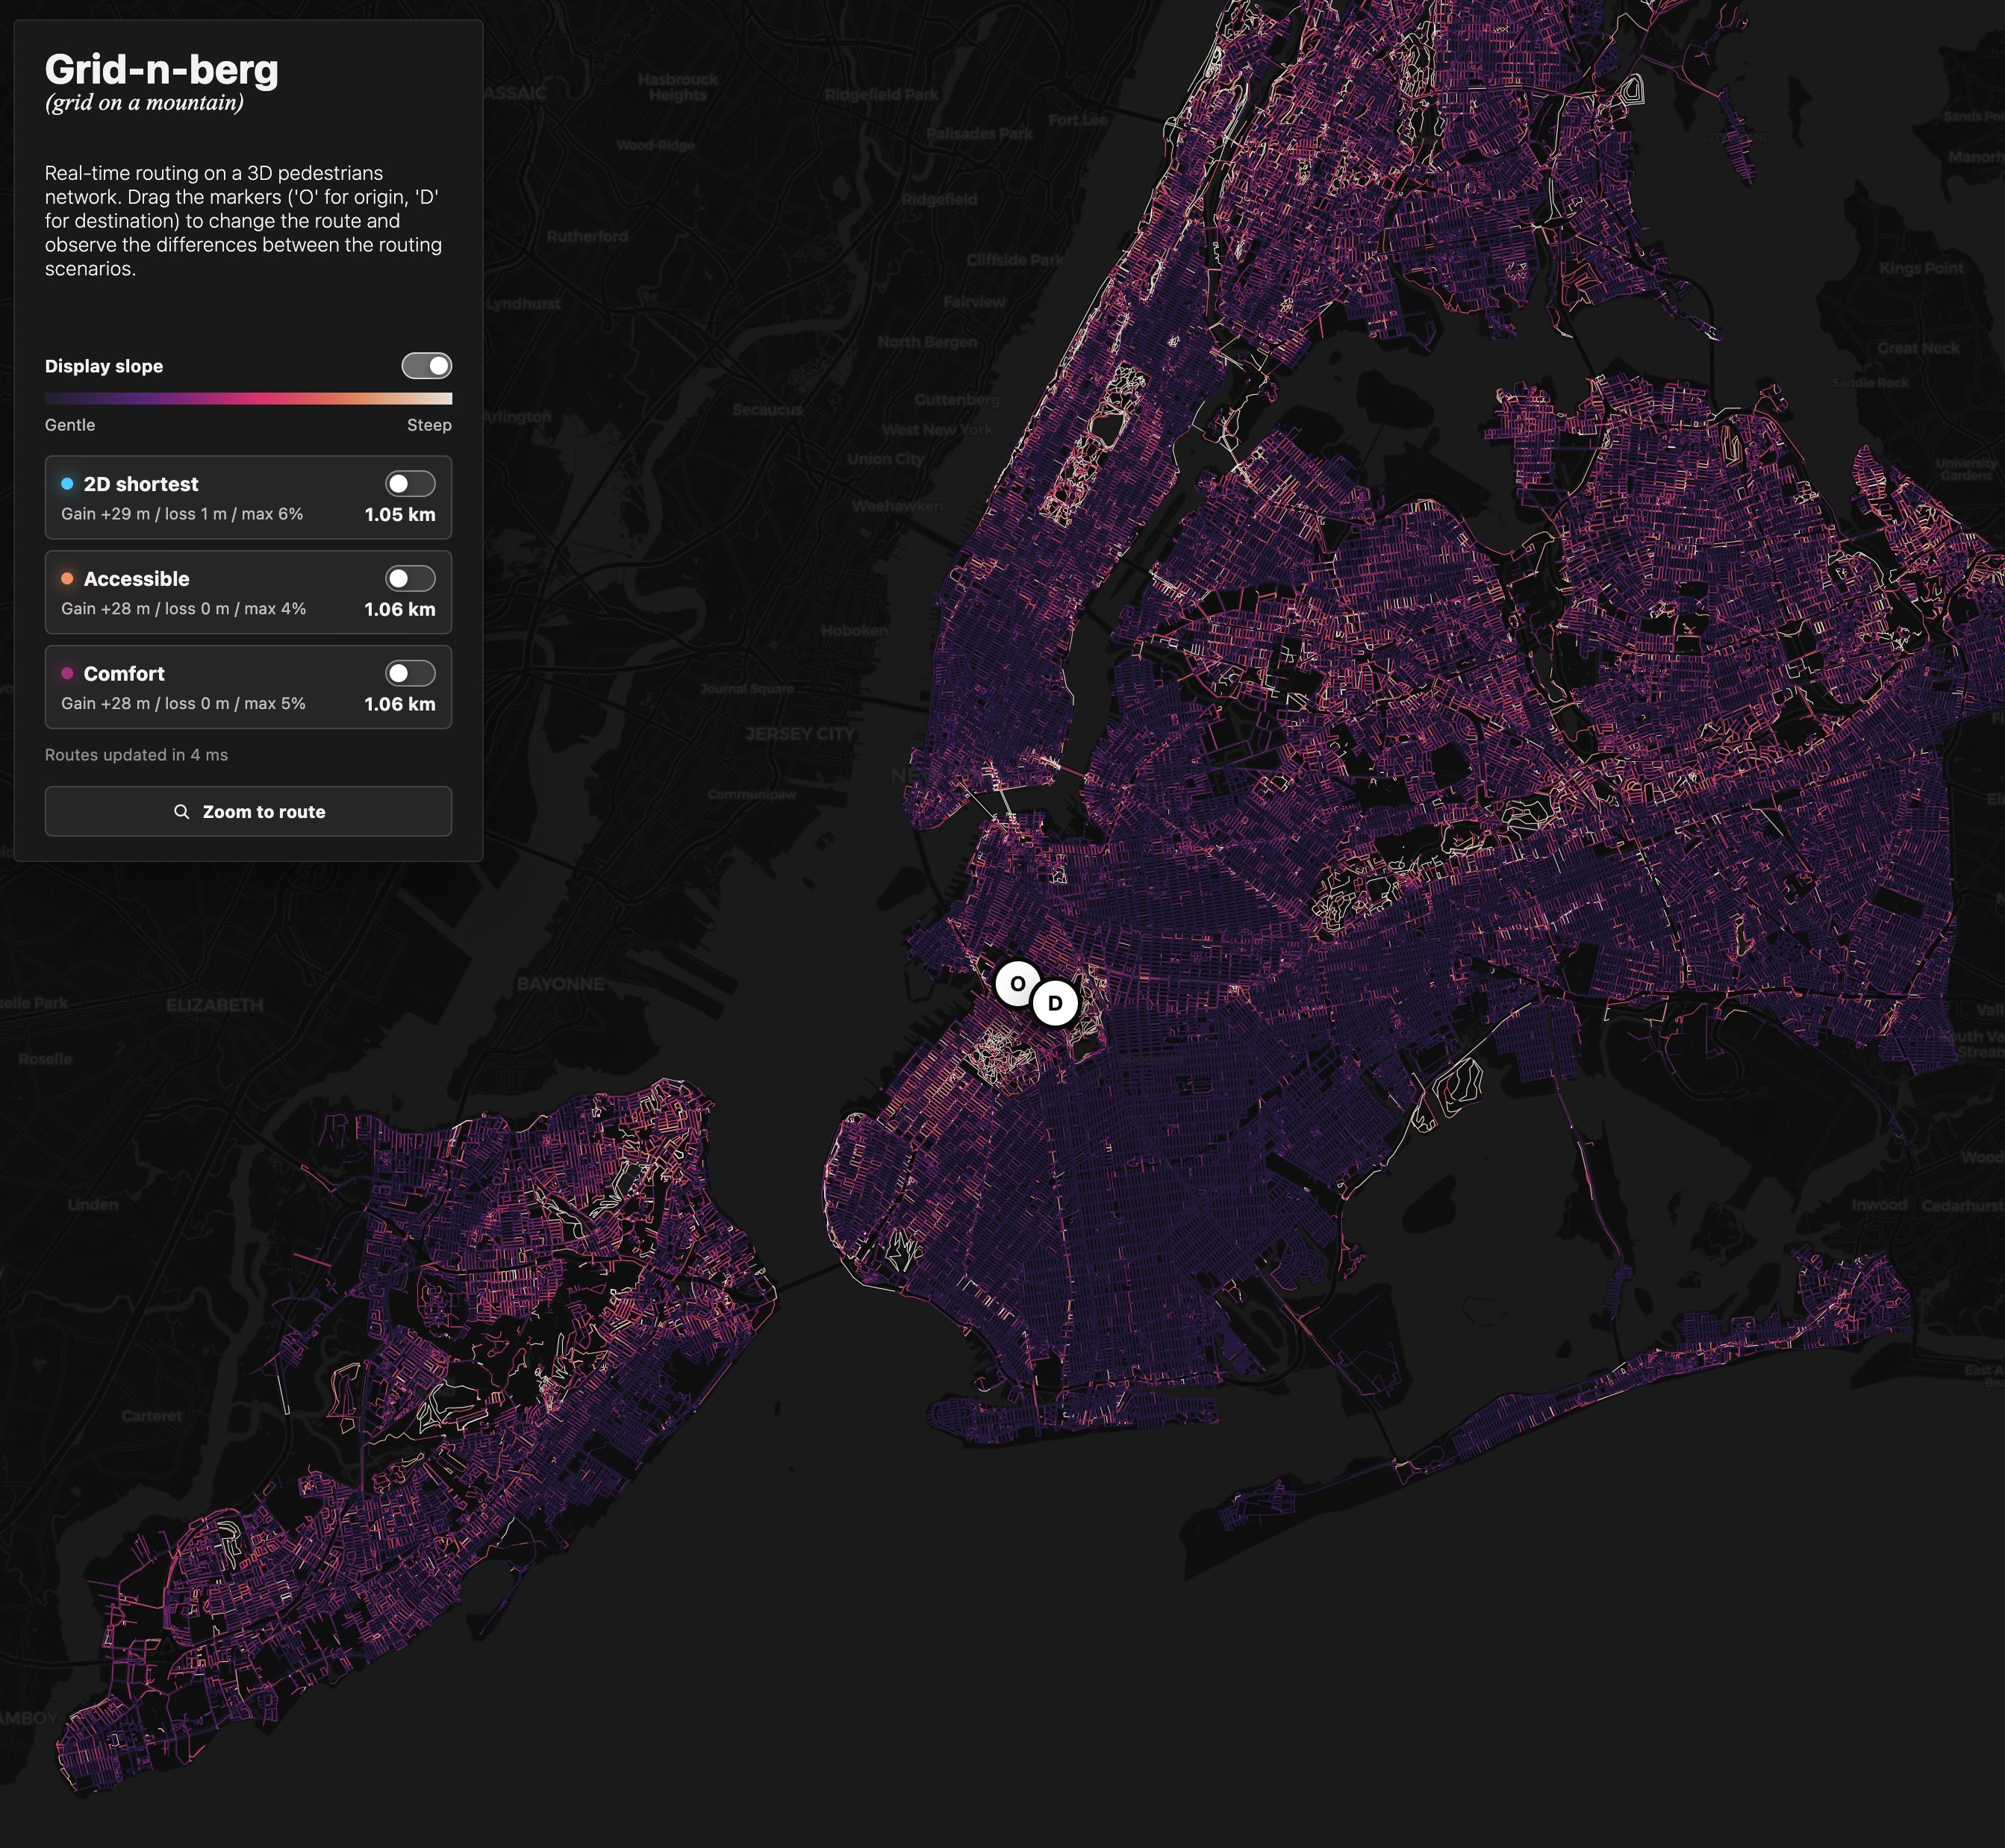
\includegraphics[width=0.96\linewidth]{gridnberg-interface.jpeg}
  \caption{The \dataset web application combines a citywide grade layer with distance-only, comfort-oriented, and accessibility-sensitive route comparison. This interface overview is illustrative and does not supply the quantitative route cases reported below; the application is not a turn-by-turn navigation service.}
  \label{fig:interface}
\end{figure}

\section{Related work}

\subsection{Open urban and pedestrian networks}

OpenStreetMap-based tools have made street-network acquisition and analysis reproducible across many cities~\citep{boeing2017osmnx,boeing2022street}. Yet street centerlines are an imperfect proxy for walking because pedestrians occupy sidewalks, crossings, paths, passages, and other surfaces that do not always follow vehicular topology. Reviews of sidewalk networks describe persistent gaps in representation, interoperability, validation, and public availability~\citep{rhoads2023sidewalk}. Recent work has developed methods for mapping pedestrian infrastructure at scale and for representing urban space as surfaces rather than only centerlines~\citep{hosseini2023mapping,barthelemy2025surfacic}. In New York,~\citep{sevtsuk2026spatial} assembled and validated NYCWalks, a detailed pedestrian network supporting citywide foot-traffic estimation. 
\\
\\
\\
\\
\\
\\
\\
\\
\\
\\
\\
\\
\\
\\
\\
\\
\\
\\
\\
\\
\\
\\
A New York-specific elevation precedent is the Robotability Score~\citep{franchi2025robotability} which derives sidewalk centerlines from Planimetric sidewalk polygons and incorporates a nondirectional local slope proxy from LiDAR into a robitic suitability index. Its published map exposes an aggregate score, not node heights, graph topology, directed edge grades, or routing costs. \dataset addresses a different research object: a route-ready NYCWalks derivative in which node elevation and direction-specific grade impedance are reusable graph attributes. It should not be described as the first New York sidewalk analysis to incorporate elevation.

\subsection{Networks beyond the plane}

Three-dimensional and multi-level pedestrian-network research shows that conventional two-dimensional representations can misstate connectivity where bridges, underground passages, elevated walkways, and vertically separated routes are common. Work in Hong Kong has formalized three-dimensional pedestrian topology and examined access in cities where ``ground'' is not a single surface \citep{sun2021connecting,zhang2022walking}. The conceptual problem differs from terrain enrichment: a topographic graph assigns height to a known path, whereas a multi-level graph must also encode vertical topology. The two problems meet around bridges, stairs, tunnels, and stacked infrastructure, where elevation assignment cannot repair an incorrect or ambiguous connection.

\subsection{Slope as impedance}

Slope-sensitive movement models extend from Tobler's hiking function and physiological work on the energy cost of inclined walking to route-choice and speed models \citep{tobler1993three,minetti2002energy,goodchild2020beyond,irmischer2018measuring}. Studies have compared distance, time, and metabolic-energy optimization; estimated walking-speed variation from terrain and fitness-tracker data; and shown that hills affect both walking and cycling choices \citep{paez2020comparing,campbell2019crowdsourced,campbell2022predicting,broach2012cycling}. These approaches are often calibrated to time, energy, or observed choice. \dataset instead provides transparent scenario scores. Its costs are intentionally legible and adjustable, but they should not be interpreted as calibrated behavioral utilities.

The ``easiest path'' and profile-routing literature is the closest methodological precedent. \citet{nourian2015easiest} combine geographic and configurational analysis for walking and cycling, while Configurbanist implements easiest-path comparison in an urban-design workflow \citep{nourian2015configurbanist}. CAPRA supports route profiling across mobility needs \citep{rahaman2017capra}; \citet{higgins2021hiking} examines terrain-aware pedestrian routing with Tobler's function. At dataset scale, \citet{bolten2021routine} derive incline-aware sidewalk accessibility measures, and newer inclusive-routing datasets combine detailed road environments with mobility-sensitive costs \citep{hosseini2024inclusive,ng2024beyond}. These studies establish that grade matters and that no single impedance function represents every pedestrian. \dataset therefore releases multiple profiles and the components needed to replace them.

\section{Data and methods}

\subsection{Source data}

The workflow combines two public sources with different geometries, coordinate systems, and semantic roles (Table~\ref{tab:sources}). The pedestrian source is the supplemental NYCWalks network created by \citet{sevtsuk2026spatial}. It contains \num{315577} LineString records representing sidewalks, crosswalks, and footpaths. The working copy is projected in EPSG:6538, whose horizontal units are metres. Only geometry is used; the source study's pedestrian-count estimates are excluded.

Elevation comes from the 2022 NYC Planimetric Database \texttt{ELEVATION} class \citep{nyc2022elevation,nyc2022capture}. The full class contains \num{1471855} three-dimensional points in EPSG:2263 with elevations referenced to NAVD88 and recorded in US survey feet. It includes ground, bridge, water, and building-roof observations. Before matching, \dataset selects the \num{387566} roadbed spot and bridge points identified by \texttt{FEATURE\_CODE=3000}, corresponding to \texttt{SUB\_FEATURE\_CODE} values 300000 and 300020. This exclusion is essential: building-roof elevations account for 73.6\pct of the full class and would contaminate pedestrian ground estimates. The current workflow converts the selected coordinates and elevations to metres using \(1\) US survey foot \(=0.3048006096\) m. It does not perform a formal coordinate transformation between the datum realizations represented by EPSG:2263 and EPSG:6538; that residual should be quantified in the next validation.

\begin{table*}[t]
  \centering
  \caption{Source datasets and their role in \dataset.}
  \label{tab:sources}
  \small
  \begin{tabularx}{\linewidth}{@{}>{\raggedright\arraybackslash}p{0.22\linewidth}>{\raggedright\arraybackslash}p{0.22\linewidth}>{\raggedright\arraybackslash}X@{}}
    \toprule
    Source                                   & Working content                                                                                    & Use and exclusions                                                                                     \\
    \midrule
    NYCWalks pedestrian network              & \num{315577} LineStrings; EPSG:6538                                                                & Supplies sidewalk, crosswalk, and footpath geometry. Foot-traffic estimates are not used.              \\
    NYC Planimetric \texttt{ELEVATION}, 2022 & \num{387566} roadbed spot and bridge points selected from \num{1471855} records; EPSG:2263; NAVD88 & Supplies local height observations. Building-roof and water observations are excluded before matching. \\
    ADA Chapter 4                            & Walking-surface and ramp grade references                                                          & Motivates the 5\pct and 8.33\pct breakpoints. It is not used to label compliance.                      \\
    \bottomrule
  \end{tabularx}
\end{table*}

The Planimetric capture rules place spot elevations along roadbeds and interior sidewalk centerlines, commonly at beginnings, midpoints, ends, and intervals no greater than 200 feet \citep{nyc2022capture}. They are therefore relevant local observations, but not continuous sidewalk surveys. In particular, they do not measure cross slope, and pedestrian or bicycle bridges may lack dedicated bridge elevation points.

\subsection{Local elevation assignment}

The source network contains \num{1248044} vertex occurrences and \num{805864} unique horizontal vertex coordinates. A regular \SI{25}{\metre} search grid indexes the selected elevation points. For every unique network vertex \(v\) with horizontal coordinate \(x_v\), the assigned elevation is the unweighted mean
\begin{equation}
  \begin{aligned}
    z_v & = \frac{1}{|P_v|}\sum_{p\in P_v} z_p,                 \\
    P_v & = \{p: \lVert x_p-x_v\rVert_2 \leq \SI{50}{\metre}\}.
  \end{aligned}
  \label{eq:elevation}
\end{equation}
A vertex is supported when \(|P_v|\geq1\). The workflow does not substitute a distant nearest neighbour because such a fallback can yield plausible-looking but locally unrelated heights. A segment is retained only when every one of its geometry vertices is supported. This rule preserves \num{313184} of the \num{315577} source segments (99.24\pct) and \num{768748} unique three-dimensional geometry vertices.

The \SI{50}{\metre} radius trades spatial specificity for source coverage. Among retained unique vertices, the median number of contributing observations is 6, with a range of 1 to 80. The median nearest contributing point is \SI{10.14}{\metre} away; the 99th percentile is \SI{36.52}{\metre}. These diagnostics describe support, not vertical accuracy. A radius sensitivity analysis and comparison against surveyed sidewalk profiles remain necessary validation steps.

\begin{figure*}[t]
  \centering
  \begin{tikzpicture}[
      node distance=4mm and 4mm,
      box/.style={draw=black!28, rounded corners=2pt, fill=black!2, align=center,
          minimum height=12mm, text width=0.15\linewidth, inner sep=4pt,
          font=\small},
      arrow/.style={-{Latex[length=2mm]}, line width=0.65pt, draw=black!55}
    ]
    \node[box] (network) {NYCWalks\\pedestrian geometry};
    \node[box, below=of network] (elev) {Roadbed and bridge\\spot elevations};
    \node[box, right=of network, yshift=-8.5mm] (match) {Unit conversion and\\50 m local mean};
    \node[box, right=of match] (retain) {Complete-support\\3D segments};
    \node[box, right=of retain] (metrics) {Directional grade,\\gain, loss, and costs};
    \node[box, right=of metrics] (release) {CSV, GeoPackage,\\analysis, and web app};
    \draw[arrow] (network.east) -- (match.west);
    \draw[arrow] (elev.east) -- (match.west);
    \draw[arrow] (match) -- (retain);
    \draw[arrow] (retain) -- (metrics);
    \draw[arrow] (metrics) -- (release);
  \end{tikzpicture}
  \caption{\dataset processing sequence. Elevation selection precedes the public matching notebook and must be reproduced explicitly in a fully automated release.}
  \label{fig:workflow}
\end{figure*}

\subsection{Segment measures and graph construction}

For a retained segment with ordered vertices \((x_i,z_i)\), horizontal length is \(L=\sum_i\lVert x_{i+1}-x_i\rVert_2\). Positive and negative elevation changes are accumulated separately over all geometry steps:
\begin{equation}
  \begin{aligned}
    G^+ & = \sum_i \max(z_{i+1}-z_i,0), \\
    G^- & = \sum_i \max(z_i-z_{i+1},0).
  \end{aligned}
\end{equation}
The public table also reports endpoint net change, endpoint-average grade, and the maximum absolute local grade among geometry steps at least \SI{1}{\metre} long. The one-metre rule prevents extremely short horizontal steps from dominating the reported local maximum. It does not currently remove those steps from \(G^+\), \(G^-\), or routing cost, a distinction revisited in Section~\ref{sec:limitations}.

Every retained physical segment is stored once with endpoint identifiers \(a\) and \(b\), then treated as two directed edges for routing. The workflow assumes every retained source segment can be traversed in both directions; \(a\) and \(b\) are storage conventions, not source access restrictions. Reversing direction exchanges \(G^+\) and \(G^-\) while preserving horizontal length and maximum absolute grade. Directional costs are stored side by side in the public segment table, avoiding duplicated geometry. Only segment endpoints become routing nodes. A further \num{581091} retained internal geometry vertices shape length and cost but cannot serve as graph junctions.

\subsection{Routing profiles}

The distance-only cost is \(C_0=L\). The other profiles use a transparent piecewise grade penalty. Let \(q^+=G^+/L\) and \(q^-=G^-/L\) be cumulative positive and negative grade ratios in a given direction. For threshold values \(g_0=0.05\) and \(g_1=1/12\), define
\begin{equation}
  \begin{aligned}
    h(q;w_m,w_s)={} & w_m\min\{\max(q-g_0,0),g_1-g_0\} \\
                    & +w_s\max(q-g_1,0).
  \end{aligned}
  \label{eq:penalty}
\end{equation}
The directional score is
\begin{equation}
  \begin{aligned}
    C=L\big[1&+h(q^+;w_{u,m},w_{u,s}) \\
         &+h(q^-;w_{d,m},w_{d,s})\big].
  \end{aligned}
  \label{eq:cost}
\end{equation}
Table~\ref{tab:profiles} lists the scenario weights. Uphill and downhill use different weights because they impose different kinds of effort and control. The accessibility-sensitive profile increases both, particularly beyond 8.33\pct. The two breakpoints provide recognizable grade references from ADA Chapter 4 \citep{usaccessboard2010ada}; they do not turn the model into an ADA evaluation. The scores are neither seconds nor joules, and the weights have not been calibrated to observed choices or a specific mobility device. Figure~\ref{fig:elevation-slope-view} shows how the web application combines assigned elevation with the penalty-relevant grade layer.

\begin{table*}[t]
  \centering
  \caption{Directional routing profiles. ``Moderate'' applies between 5\pct and 8.33\pct; ``steep'' applies above 8.33\pct.}
  \label{tab:profiles}
  \small
  \begin{tabular}{@{}lrrrrl@{}}
    \toprule
    Profile                 & \multicolumn{2}{c}{Uphill weights} & \multicolumn{2}{c}{Downhill weights} & Interpretation                                    \\
    \cmidrule(lr){2-3}\cmidrule(lr){4-5}
                            & Moderate                           & Steep                                & Moderate       & Steep &                          \\
    \midrule
    Distance-only           & 0                                  & 0                                    & 0              & 0     & Horizontal shortest path \\
    Comfort-oriented        & 8                                  & 30                                   & 2              & 8     & Moderate grade aversion  \\
    Accessibility-sensitive & 20                                 & 80                                   & 12             & 50    & Strong grade aversion    \\
    \bottomrule
  \end{tabular}
\end{table*}

\begin{figure*}[t]
  \centering
  \includegraphics[width=0.90\linewidth]{gridnberg-elevation-slope-3d.png}
  \caption{Vertically exaggerated three-dimensional view of the \dataset network in and around Central Park. Three linked attributes are visible simultaneously: assigned network elevation through vertical position; topographic relief through an accentuated vertical scale; and penalty-relevant slope severity through the color of each segment's maximum local absolute grade. Purple lies below the 5\pct penalty breakpoint, magenta and pink span the moderate range, and orange to white marks increasingly steep links beyond 8.33\pct. Color is a nondirectional diagnostic; routing costs remain direction-specific and are calculated from cumulative gain and loss.}
  \label{fig:elevation-slope-view}
\end{figure*}

\section{Data records and technical validation}

\subsection{Released records}

The analytical release contains \num{187657} endpoint nodes and \num{313184} physical segments, equivalent to \num{626368} directed edges. Their summed horizontal length is \SI{20076.08}{\kilo\metre}. This total is not street mileage: separately mapped sidewalk sides, crossings, paths, and multi-vertex features all contribute. Table~\ref{tab:records} summarizes the principal products. CSV files are the authoritative tabular outputs, but the GeoPackage is required to inspect the internal three-dimensional geometry from which gain, loss, and cost were calculated. Browser JSON and GeoJSON are display and routing derivatives.

\begin{table*}[t]
  \centering
  \caption{Principal release products.}
  \label{tab:records}
  \small
  \begin{tabularx}{\linewidth}{@{}p{0.30\linewidth}p{0.18\linewidth}X@{}}
    \toprule
    Record                        & Size                & Contents and intended use                                                                         \\
    \midrule
    \texttt{routing\_nodes.csv}   & \num{187657} rows   & Node identifier, EPSG:6538 coordinates, and assigned elevation in metres.                         \\
    \texttt{routing\_network.csv} & \num{313184} rows   & Endpoint identifiers, length, endpoint elevations, grade summaries, and costs in both directions. \\
    Routing GeoPackage            & 2 layers            & Three-dimensional segment geometry and routing nodes for GIS inspection.                          \\
    Browser derivatives           & JSON and GeoJSON    & Compact graph, display geometry, and route attributes used by the web application.                \\
    Workflow and audit scripts    & Notebook and Python & Elevation assignment, exports, descriptive statistics, and illustrative route reconstruction.     \\
    \bottomrule
  \end{tabularx}
\end{table*}

The segment-length median is \SI{32.07}{\metre}; the 95th percentile is \SI{218.96}{\metre}. Node elevation ranges from \SI{-0.33}{\metre} to \SI{121.09}{\metre}, with a median of \SI{12.97}{\metre}. Median absolute endpoint-average grade is 0.58\pct and the 95th percentile is 4.74\pct. The maximum local absolute grade has a median of 0.88\pct and a 95th percentile of 10.60\pct. In total, \num{40064} segments (12.79\pct) contain a reported local grade of at least 5\pct, \num{21430} (6.84\pct) reach at least 8.33\pct, and \num{14895} (4.76\pct) receive a slope penalty in at least one direction.

The graph has 256 connected components, compared with 203 in the source graph. Its largest contains \num{158110} nodes (84.25\pct) and \num{266698} physical edges; Staten Island and the Rockaway peninsula form the next two largest. Some additional fragmentation is produced by the complete-support rule. On the Marine Parkway and Cross Bay bridges, five source vertices miss the \SI{50}{\metre} threshold by only 1.27--5.49 m, separating the Rockaways. A coverage-only audit at \SI{55}{\metre} reconnects that component, but also increases the risk of mixing vertically distinct observations. This audit was not used to rebuild the release. The graph also contains two self-loops and \num{4363} endpoint pairs with parallel segments. Parallel links can be valid when distinct pedestrian facilities share endpoints; routing implementations should therefore use a multigraph or retain segment identifiers.

\subsection{Reconstruction and quality control}

Technical validation proceeded at three levels. First, reconstruction from the archived sources produces the released coverage: \num{781900} of \num{805864} unique source vertices receive local support, and the complete-support rule retains \num{313184} segments. Second, a check of 63 released node elevations recalculated the local mean directly from the source spot and bridge observations; all values match the released node table within floating-point rounding. Repeating the calculation with the unfiltered Planimetric class produces large errors near buildings, confirming the necessity of the feature-code filter. Third, the public analysis script recalculates row counts, distributions, graph structure, directional asymmetry, and representative routes from the released CSV and browser graph.

These checks verify internal transformation, not sidewalk-elevation truth. Distributional review identifies a small but important implausible tail. There are \num{470} segments (0.15\pct) with a reported local absolute grade of at least 100\pct. At Dyckman Fields, one \SI{0.34}{\metre} segment changes \SI{4.74}{\metre} in elevation: because its horizontal step is below the one-metre reporting threshold, its maximum local grade is reported as zero, while its accumulated gain still produces an extreme cost. Such records may arise from stairs, vertical or multi-level connections, geometry artifacts, or mismatched elevation support. They are retained in this initial research release to make the failure mode visible, but they should be flagged or revised before safety-critical routing.

\section{Illustrative route comparisons}

Figure~\ref{fig:routes} compares the three profiles for two origin--destination pairs selected to illustrate distinct behavior. In St.~George, Staten Island, the distance route is \SI{1.76}{\kilo\metre} with \SI{48}{\metre} of endpoint-derived cumulative gain and a maximum reported local grade of 35.5\pct. The comfort-oriented route is 5.5\pct longer but reduces the corresponding gain to \SI{43}{\metre} and the maximum to 14.2\pct. The accessibility-sensitive route follows nearly the same corridor. This is the intended use of the profiles: expose a measurable distance--grade trade-off, not declare a universal optimum.

The Morningside Heights--Harlem case is diagnostic. Its distance route encounters a segment with a reported local grade of 209.2\pct; both slope-sensitive profiles take a 2.3\pct detour and reduce the route maximum to 10.2\pct. The route engine behaves consistently with the assigned cost, but the avoided value is physically implausible for an ordinary walkway and demands source review. A useful topographic dataset should reveal this distinction: optimization can route around an anomalous edge without establishing that the anomaly represents terrain.

\begin{figure*}[t]
  \centering
  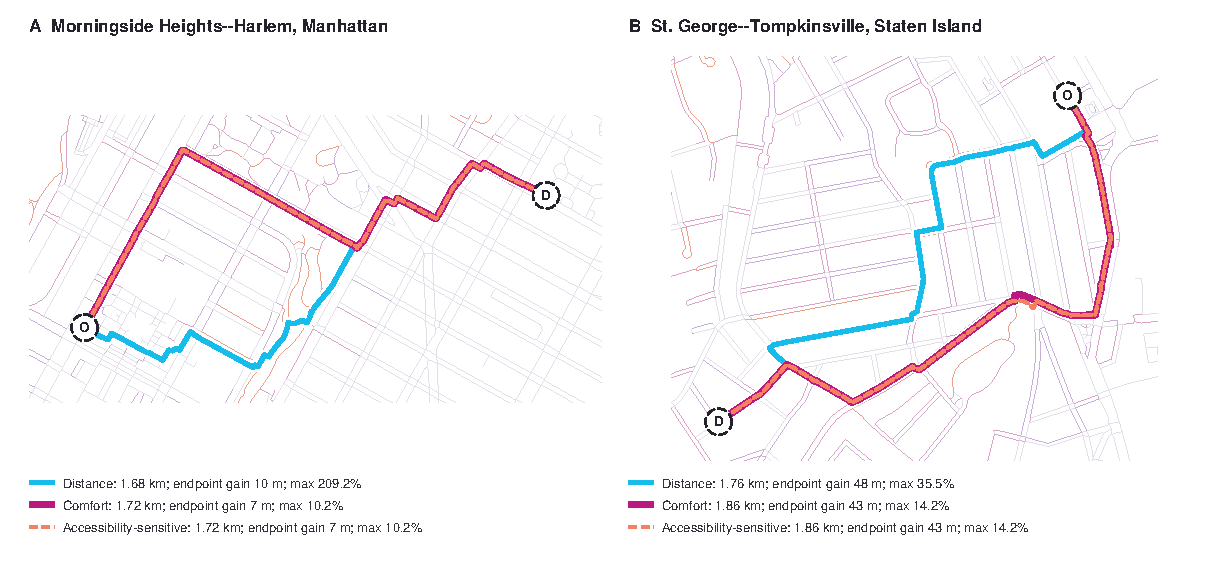
\includegraphics[width=\linewidth]{route_cases.pdf}
  \caption{Illustrative route comparisons reconstructed from the released browser graph. Panel A shows a diagnostic case in Morningside Heights--Harlem, where an implausibly steep source-derived edge changes route choice. Panel B shows a more plausible distance--grade trade-off in St.~George--Tompkinsville. Gain is summed from endpoint changes in the current application, while the routing cost uses changes across all intermediate geometry vertices. Maximum grade is the largest released local-grade value along each route.}
  \label{fig:routes}
\end{figure*}

The data support uses beyond pairwise navigation. Researchers can test how terrain changes network centrality or pedestrian catchments; compare the planar and grade-sensitive reach of transit, parks, schools, cooling centers, or public facilities; identify where steep links concentrate route burden; and examine whether alternative network improvements reduce grade exposure. Directed costs make uphill and downhill catchments non-reciprocal. The components also support sensitivity studies in which empirically calibrated time, metabolic-energy, wheelchair, cycling, or user-specific functions replace the provided scenarios \citep{paez2020comparing,greenberg2020physical,ng2024beyond}.

The most informative edge cases are not limited to steep hills. Near Queensboro Bridge and the RFK Bridge on Randall's Island, several extreme records result when ground observations around paths enter the same moving window as road or bridge-deck observations tens of metres higher. Stairs may be geometrically valid but inappropriate for some users; very short features can amplify noise; underpasses and elevated paths can be topologically connected in two dimensions while vertically separate; and a \SI{50}{\metre} mean can smooth a sharp local transition. These cases make \dataset useful as a diagnostic object for studying how elevation sources and pedestrian topology interact, not only as a finished route product.

\section{Limitations and next validation steps}
\label{sec:limitations}

\dataset has five principal limitations. First, the elevation field is a local mean of municipal spot observations rather than a surveyed longitudinal profile of each pedestrian facility. The method can smooth terrain, mix nearby vertical levels, and propagate a discordant observation. A systematic comparison of 25, 50, and \SI{75}{\metre} radii and validation against independent profiles are priorities.

Second, the source graph is assumed to represent walkable connectivity. Elevation enrichment cannot determine whether a link is legally accessible, temporarily obstructed, or correctly connected across stacked infrastructure. It also does not distinguish streets, ramps, stairs, and bridges in the released cost logic.

Third, the routing profiles are heuristic. The terms ``comfort-oriented'' and ``accessibility-sensitive'' denote relative scenario weights, not measured comfort, travel time, energy, universal design, or the needs of a particular pedestrian. The dataset does not measure cross slope, curb ramps, sidewalk width, surface condition, obstacles, lighting, signal timing, construction, or snow. It must not be used to certify ADA compliance.

Fourth, the one-metre safeguard is inconsistent across outputs: it limits the reported maximum local grade but does not remove short-step elevation changes from gain, loss, or cost. The implausible tail should be addressed through a documented policy that preserves legitimate stairs and vertical links while flagging or correcting artifacts. Source record identifiers and per-vertex support diagnostics should also be carried into the public tables to make this review traceable. The current \texttt{network\_record\_number} is a generated sequence rather than an original source identifier. The web application's three-dimensional view linearly interpolates endpoint elevations, and its gain/loss summary uses endpoint changes; neither substitutes for the internal geometry used by routing.

Fifth, the present repository does not yet provide a fully automated source-acquisition and preprocessing stage. The elevation subtype filter is applied before the public notebook, and the source files are excluded because of their size. A publication release should add a versioned environment, scripted source retrieval or clear manual acquisition instructions, explicit feature-code filtering, a license, checksums, and a persistent archive DOI. These are release-engineering limitations rather than hidden analytical assumptions, and they are recorded in the accompanying paper checklist.

\section{Conclusion}

\dataset makes terrain an explicit, inspectable part of a citywide pedestrian graph for New York City. It documents how local elevations are assigned, how direction-specific grade costs are constructed, and how route choice changes under three transparent scenarios. The release also exposes unresolved cases where topography, vertical infrastructure, and data artifacts are difficult to distinguish. Its immediate value is therefore twofold: it enables reproducible terrain-aware analysis, and it provides a concrete basis for improving how pedestrian networks represent elevation. The next version should pair the open transformation with stronger outlier handling, radius sensitivity, field validation, and user-calibrated impedance models.

\section*{Data and code availability}

The data, code, QGIS project, and web application are available at \url{https://github.com/RELNO/gridnberg}. The public application is deployed at \url{https://arielnoyman.com/gridnberg/}. The two CSV files under \texttt{outputs/} are the authoritative public tables. The source NYCWalks network and NYC Planimetric elevation points remain governed by their respective providers and are cited separately. This initial preprint describes the version distributed through the project repository.

\section*{Author contributions}

Ariel Noyman: Conceptualization, methodology, software, data curation, formal analysis, visualization, writing--original draft, and writing--review and editing.

\section*{Acknowledgments}

The author thanks Andres Sevtsuk and collaborators for releasing the pedestrian-network work on which \dataset builds, and the City of New York for maintaining the Planimetric Database.

\section*{AI assistance disclosure}

AI-assisted tools were used to support literature discovery, code inspection, descriptive analysis, and editorial drafting. The author is responsible for source verification, methodological claims, analyses, and the final text.

\balance
\printbibliography

\end{document}
